\documentclass[12pt,a4paper]{article}
\usepackage[utf8]{inputenc}
\usepackage[english,russian]{babel}
\usepackage{indentfirst}
\usepackage{misccorr}
\usepackage[warn]{mathtext}
\usepackage{subcaption}
\captionsetup{compatibility=false}
\usepackage{graphicx}
\usepackage{wrapfig}
\usepackage{amsmath}
\usepackage{floatflt}
\usepackage{float}
\usepackage{amssymb}
\usepackage{color}
\usepackage{lscape}
\usepackage{hvfloat}
\usepackage{amsfonts}
\usepackage{euscript}
\usepackage{multicol}
\usepackage{multirow}


\graphicspath{{pictures/}}
\DeclareGraphicsExtensions{.png,.jpg, .jpeg}
\usepackage[left=20mm, top=20mm, right=20mm, bottom=20mm, footskip=10mm]{geometry}
\linespread{1.3}

\begin{document}
\begin{titlepage}
  \begin{center}
    \large
    Московский физико-технический институт
    
    (Национальный исследовательский университет)
    \vspace{0.5cm}

   
    \vspace{0.25cm}
 
    \vfill
 
    \vfill

    \textsc{\bf{Вопрос по выбору}}\\[5mm]
    
    {\LARGE Эффект Фарадея}
  \bigskip
    \vfill
    
\end{center}
\vfill
\begin{flushright}

    Выполнила студентка Б04-901 группы

    Гарибова Лейла

\end{flushright}

\bigskip


\vfill

\begin{center}

  Долгопрудный, 2021 г.
\end{center}
\end{titlepage}
\newpage


\subsubsection*{Цель работы: } Изучить эффект Фарадея.

\subsection*{Вывод формулы}
Фарадеем было установлено, что при распространении линейно поляризованного света через среду, находящуюся в мгнитном поле,  наблюдается вращение плоскости поляризации. 

Было установлено, что угол поворота не зависит от направления распространения света и пропорционален величине поля и длине пути света в веществе:
 \begin{equation*}
     \varphi = VLB.
 \end{equation*}
\begin{figure}[H]
\begin{center}
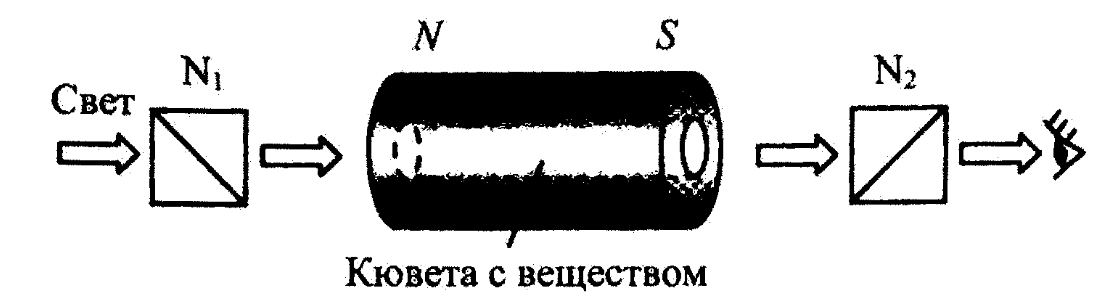
\includegraphics[width = 0.7\textwidth]{оф.PNG}
\caption{Схема опыта по наблюдению эффекта Фарадея. Кювета с веществом находится в продольном магнитном поле. До и после кюветы свет пропускается через николи со взаимно перпендикулярными осями}
\end{center}
\end{figure}
 Запишем уравнение движения электрона в поле волны ($E$) и в постоянном магнитном поле ($B$):
 \begin{equation*}
     m\Ddot{\textbf{r}} = -k\textbf{r} + e\textbf{E} + \frac{e}{c}\Dot{\textbf{r}} \times \textbf{B}
 \end{equation*}
Мы пренебрегли трением, считая, что все характерные частоты находятся далеко от линий поглощения излучения веществом. Введем циклотронную частоту:
 \begin{equation*}
     \Omega = -\frac{e\textbf{B}}{mc},
 \end{equation*}
дающую угловую скорость вращения электрона. Тогда уравнение примет вид:
 \begin{equation*}
     \Ddot{\textbf{r}}  + \Omega \times\Dot{\textbf{r}} + \omega_{0}^2 \textbf{r} = e \textbf{E}.
 \end{equation*}
 Пусть волна распространяется в направлении оси z, куда направлено также магнитное поле. При этом
  \begin{equation*}
  \Omega_{z} = -\frac{e\textbf{B}}{mc} = \frac{|e|B}{mc} = \Omega > 0.
 \end{equation*}
 Если волна имеет линейную поляризацию, то ее можно расписать как сумму двух круговых поляризаций:
  \begin{align*}
     &E_x = E_0 \cos{\omega t},\\
     &E_y = \pm E_0 \sin{\omega t}
  \end{align*}
    
 
 Во втором равенстве знаки отвечают за правую и левую поляризации соответсвенно.
 
 Таким образом, получаем следующую систему уравнений:
   \begin{align*}
     &\Ddot{x} - \Omega\Dot{y} + \omega_{0}^2 x = E_0 \cos{\omega t},\\
     &\Ddot{y} - \Omega\Dot{x} + \omega_{0}^2 y =\pm E_0 \sin{\omega t}
  \end{align*}
Решение этой системы имеет вид:
   \begin{align*}
     &x = \frac{e/m}{\omega^2_0 - \omega^2 \mp \Omega\omega}E_x,\\
     &y = \frac{e/m}{\omega^2_0 - \omega^2 \mp \Omega\omega}E_y.
  \end{align*}
Поскольку дипольный момент, приобретаемый электроном, равен $\textbf{p} = e\textbf{r}$, а вектор поляризации системы -- $\textbf{P} = N\textbf{p} = \alpha\textbf{E}$, где $N$ -- концентрация электронов в среде, то диэлектрическая проницаемость среды оказывается равной:
\begin{equation*}
    \varepsilon_{\pm} = 1 + \frac{\omega^2_p}{\omega^2_0 - \omega^2 \mp \Omega\omega}
\end{equation*}
Здесь величина $\omega^2_p = \sqrt{4 \pi N e^2/m}$ есть плазменная частота.

Из полученной формулы следует, что показатель преломления $n = \sqrt{\varepsilon}$ зависит от того, какова поляризация волны (левая или правая).

Далее учтем, что частоты света порядка $\omega \approx 10^{15}\:\: \mbox{с}^{-1}$, а циклотронная частота даже для сильных полей составляет $\Omega \approx 10^{10}\:\: \mbox{с}^{-1} \ll \omega$. Поэтому $\omega^2 \pm \omega \Omega \approx (\omega \pm \Omega/2)^2$. Таким образом, для показателя преломления волн с левой и правой поляризациями в присутствии магнитного поля получаем выражение
\begin{equation*}
    n_{\pm} = \sqrt{1 + \frac{\omega^2_p}{\omega^2_0 -  (\omega \pm \Omega/2)^2}}.
\end{equation*}
Пусть $n(\omega)$ -- частотная зависимость показателя преломления среды. Тогда:
\begin{equation*}
    n_l = n(\omega + \Omega/2),\: n_r = n(\omega - \Omega/2),\: n_l - n_r \approx \Omega \frac{dn}{d\omega}
\end{equation*}
Угол поворота плоскости поляризации($\alpha$ - вращательная постоянная):
\begin{equation*}
    \varphi = \alpha L = \frac{\pi}{\lambda}\Omega \frac{dn}{d\omega} L = VLB,
\end{equation*}
Для постоянной Верде получаем выражение:
\begin{equation*}
    V = \frac{\pi e}{\lambda m c}\frac{dn}{d\omega} = \frac{|e|}{2mc^2}\lambda \frac{dn}{d \lambda} ,
\end{equation*}

\subsection*{Применение}
На основе эффекта Фарадея разработаны магнитооптические методы исследования тонких магнитных пленок, пропускающих свет. Такие пленки состоят из множества магнитных доменов микронных размеров. Домены являются сами источниками магнитного поля, поэтому при прохождении через домен плоскость поляризации света поворачивается. угол поворота будет зависит от ориентации домена. Поэтому амплитуда волны, прошедшей затем через анализатор, будет промодулирована в плоскости, параллельной пленке. Изучая распределение интенсивности света, можно делать выводы о магнитной структуре пленок.

Широкое распространение получили оптические изоляторы, пропускающие свет лишь в одном направлении. Основу их конструкции составляет магнитооптическая ячейка Фарадея, помещенная между двумя поляроидами.

Ячейка, выполненная в виде модуля, содержит прозрачное вещество и источник продольного магнитного поля. Пусть при прохождении через эту ячейку плоскополяризованного света плоскость поляризации поворачивается на угол $\varphi$. Если теперь эту ячейку поместить между двумя поляроидами, главные плоскости которых тоже будут повернуты на угол $\varphi$, то эта система будет пропускать плоскополяризованный свет преимущественно лишь в одном направлении.

Такой изолятор, в частности, используется в волоконных кольцевых лазерах.
\end{document}